\section{Spannungsfolger mit uA741}
\subsection{Aufgabenstellung}
Die Offsetspannung des Operationsverstärkers ist mit dem Tischmultimeter zu messen, dabei ist mittels eines Potentiometers ein Offsetabgleich vorzunehmen. Danach soll das Gehäuse mit Kältespray abgekühlt werden und die damit verschobene Offsetverschiebung aufzunehmen. 

Die Grenzfrequenz dieser Schaltung ist zu bestimmen und mit einer PSPICE Simulation zu vergleichen. Dabei sollte eine Eingangsspannung mit $V_{PP} = 100 \rm mV$ verwendet werden. 

Der Aussteuerbereich bei einer Eingangsfrequenz von $f=1 \rm kHz$ ist zu bestimmen, dabei sind die Messungen sowohl mit eine Last von $R_{Last} = 2 \rm k\Omega$ als auch ohne Last vorzunehmen. Dafür ist die Amplitude der Eingangsspannung schrittweise zu erhöhen bis eine deutliche Übersteuerung in beiden Halbwellen zu sehen ist. Für diesen Zweck ist die Versorgungsspannung auf $V_{CC} = 10\rm V$ und $V_{EE} = -10 \rm V$ zu verringern. 

Danach ist die negative Versorgungsspannung auf $V_{EE} = -5V$ zu verringern und das daraus resultierende Verhalten zu dokumentieren.

Durch anlegen einer Rechteckspannung ist die Slew Rate des Verstärkers zu bestimmen. Diese ist sowohl mit einem Lastwiderstand von $R_{Last} = 2\rm k\Omega$, als auch mit einer kapazitiven Last von $C_{Last} = 100 \rm nF$ zu bestimmen. 

Durch Kenntnis der maximalen Slew Rate ist nun die sinusförmige Spannung am Eingang anzulegen, welche gerade noch unverzerrt übertragen werden kann. Ausgehend von dieser Spannung ist nun die Frequenz schrittweise zu erhöhen bis eine deutliche Verzerrung zu erkennen ist. 
\begin{figure}[H]
    \centering
    \begin{circuitikz}[]
        \draw (0,0) node[op amp] (opamp) {$\mu A 741$};
        \draw (opamp.up) --++(0,0.5) node[vcc]{$V_{CC}$};
        \draw (opamp.down) --++(0,-0.5) node[vee]{$V_{EE}$};
        \draw (opamp.+) to[short,-o] ++(-2,0) node[left] {$U_{In}$};
        \draw (opamp.out) to[short,-o] ++(3,0) node[right] {$U_{a}$};
        \draw (opamp.-) to[short] ++(-1,0)
            to[short] ++(0,2)
            to[short] ++(6,0)
            to[short,-*] ++(0,-2.5);
        \draw (0.3,0.3) to[short] ++(0,0.5)
            to[short] ++(2.5,0)
            to[short] (2.8,-1)
            to[pR, name=offsetPoti] ++(-2,0)
            to[short] ++(-0.5,0)
            to[short] (0.3,-0.3);
        \draw (offsetPoti.wiper) node[vee]{$V_{EE}$};
        
        \end{circuitikz}
    \caption{Spannungsfolger mit Offsettrimmer}
    \label{fig:Spannungsfolger_Schaltung}
 \end{figure}


\subsection{Messaufbau}
Um alle gegebene Aufgabenstellungen erfüllen zu können, wurde die Schaltung mit zwei verschiedenen Messbeschaltungen versehen. 

zur Bestimmung der Offsetspannung wurde der Eingang der Schaltung mit Masse verbunden. Danach wurde die Ausgangsspannung mit dem Tischmultimeter gemessen und aufgezeichnet.

Im zweiten Aufbau wurde der Eingang mit einem Signagenerator betrieben und Ein- und Ausgang mit dem Oszilloskop gemessen. Für bestimmte Messungen wurde der Ausgang zusätzlich mit einem $R_{Last} = 2k\Omega$ und einem $C_{Last} = 100nF$ belastet.
\begin{figure}[H]
    \centering
    \begin{circuitikz}[]
        \draw (0,0) node[op amp] (opamp) {$\mu A 741$};
        \draw (opamp.up) --++(0,0.5) node[vcc]{$V_{CC}$};
        \draw (opamp.down) --++(0,-0.5) node[vee]{$V_{EE}$};
        \draw (opamp.+) to[short,-o] ++(-1,0) 
            %%Einfügen der Messschaltung
            to[short,o-o] ++(0,-1) node[ground] {};
        \draw (opamp.out) to[short,-o] ++(3,0)
            %Einfügen der Messchaltung
            to[voltmeter,o-o] ++(0,-2) node[ground]{};
        \draw (opamp.-) to[short] ++(-1,0)
            to[short] ++(0,2)
            to[short] ++(6,0)
            to[short,-*] ++(0,-2.5);
        \draw (0.3,0.3) to[short] ++(0,0.5)
            to[short] ++(2.5,0)
            to[short] (2.8,-1)
            to[pR, name=offsetPoti] ++(-2,0)
            to[short] ++(-0.5,0)
            to[short] (0.3,-0.3);
        \draw (offsetPoti.wiper) node[vee]{$V_{EE}$};
        
        \end{circuitikz}
    \caption{Spannungsfolger, Messaufbau zur Offsetbestimmung, $V_{CC} = 15\rm V$, $V_{EE} = -15\rm V$}
    \label{fig:Spannungsfolger_Messaufbau_Offset}
 \end{figure}

\begin{figure}[H]
    \centering
    \begin{circuitikz}[]
        \draw (0,0) node[op amp] (opamp) {$\mu A 741$};
        \draw (opamp.up) --++(0,0.5) node[vcc]{$V_{CC}$};
        \draw (opamp.down) --++(0,-0.5) node[vee]{$V_{EE}$};
        \draw (opamp.+) to[short,-o] ++(-1,0) 
            %%Einfügen der Messschaltung
            to[sV=CH1, color=white, name=S1,o-o] ++(0,-2) node[ground] {}
            to[short,o-] ++(-2,0)
            to[sV] ++(0,2)
            to[short,-o] ++(2,0);
        \draw (opamp.out) to[short,-o] ++(3,0)
            %Einfügen der Messchaltung
            to[sV=CH2, color=white, name=S2,o-o] ++(0,-2) node[ground]{};
        \draw (opamp.-) to[short] ++(-1,0)
            to[short] ++(0,2)
            to[short] ++(6,0)
            to[short,-*] ++(0,-2.5);
        \draw (0.3,0.3) to[short] ++(0,0.5)
            to[short] ++(2.5,0)
            to[short] (2.8,-1)
            to[pR, name=offsetPoti] ++(-2,0)
            to[short] ++(-0.5,0)
            to[short] (0.3,-0.3);
        \draw (offsetPoti.wiper) node[vee]{$V_{EE}$};
        \myscope{S1}{0}
        \myscope{S2}{0}
        \end{circuitikz}
    \caption{Spannungsfolger, Messaufbau zur Bestimmung des zeitlichen Verhaltens}
    \label{fig:Spannungsfolger_Messaufbau_Offset}
 \end{figure}

\subsection{Messergebnisse}
Bei der Messung der Offsetspannung ohne dem Einbau eines Trimmers zur Anpassung wurde eine Spannung von $V_{IO} = 1,792 mV$ gemessen. Diese Messung konnte mittels des Datenblattes verifiziert werden. Laut diesem sollte die Offsetspannung zwischen 1mV und 5mV liegen.\cite[6]{ti:ua741}

Nun wurde der mithilfe des Trimmers auf eine Offsetspannung von $V_{IO Trimm} = 160 \mu V$ verringert. Durch abkühlen mit einem Kältspray wurde zunächst nur wenig Änderung am Ausgang beobachtet, jedoch erhöhte sich der Offset nach einigen Sekunden signifikant, bis er ein Maximum von $V_{IO} = 2,2mV$ erreichte. 

Wie in Abbildung \ref{fig:Bode_Folger_ua741} zu sehen ist, beträgt die Grenzfrequenz der Schaltung $f_C=850KHz$. Das ist ungefähr 150KHz weniger als durch Angaben im Datenblatt, sowie der Simulation zu erwarten wäre. Die Begründung für dieses Phänomen liegt wahrscheinlich in der kapazitiven Belastung der Schaltung durch das Messequipment, sowie die kleinen Leckströme die über die Kapazitäten des Steckbretts fließen und der nicht-idealen Entkopplung der Schaltung durch den Aufbau am Steckbrett. 
\begin{figure}[H]
    \centering
    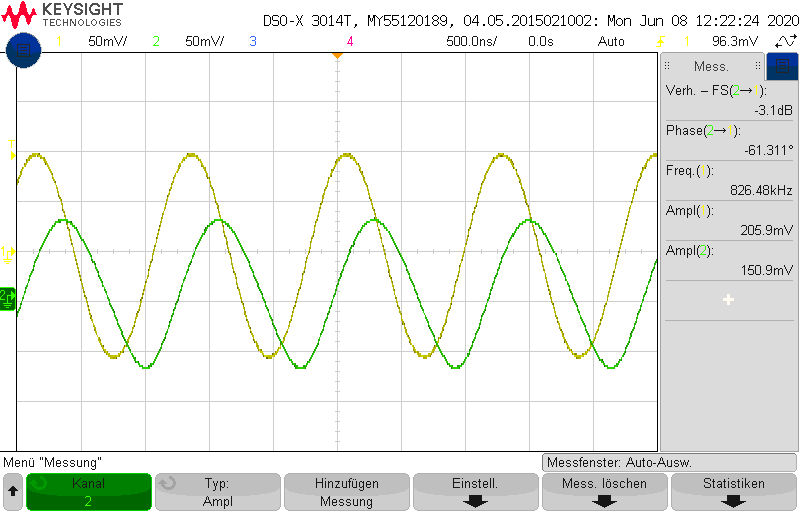
\includegraphics[width=\costumPicWidth]{Lab_1/Messungen/Folger/fg.png}
    \caption{Folgerschaltung bei der Grenzfrequenz}
    \label{fig:fg_Folger_ua741}
\end{figure}
\input{}
In \autoref{fig:fg_Folger_ua741} ist zu sehen, dass die Grenzfrequenz dieser Schaltung bei circa $f_g=826,48\kHz$ liegt. Im Datenblatt ist eine typische Grenzfrequenz bei Unity-Gain von $f_g=1\MHz$(\cite[9]{ti:ua741}) angegeben. Auch in der Simulation lag die die Grenzfrequenz bei $1\MHz$. Die Abweichung zwischen gemessenen und Werten im Datenblatt kann an der parasitären Kapazitäten im Steckbrett erklärt werden. Diese erzeugen vermutlich in der Feebackleitung durch einen kleinen Leitungswiderstand und eine winzige Kapazität einen Tiefpass erster Ordnung. Die genauen \glqq Bauteilwerte\grqq dieser Effekte wurden nicht gemessen, da sie ohnehin nicht vermeidbar sind in diesem Aufbau und die Abweichung auch nicht riesig ist und in weiteren Übungen zu Problemen führen würden.

\begin{figure}[H]
    \centering
    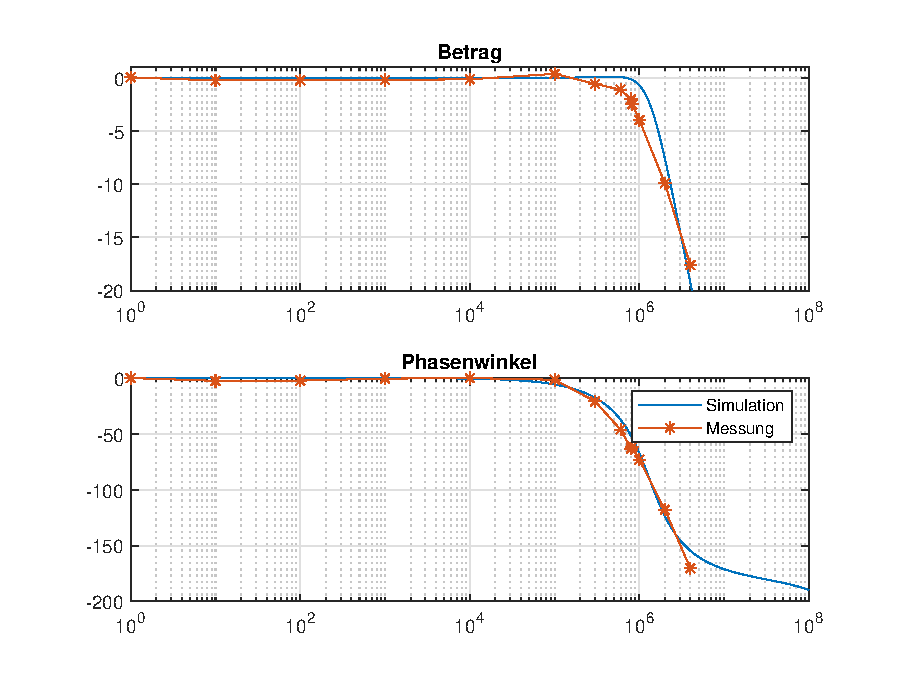
\includegraphics[width=\costumPlotWidth]{Lab_1/Plots/Folger.eps}
    \caption{Bodediagramm der Folgerschaltung, $V_{inPP}=100mV$, $V_{CC}=-V_{EE}=15V$}
    \label{fig:Bode_Folger_ua741}
\end{figure}

\begin{table}[H]
\centering
\caption{Aussteuerbereich,  $V_{CC}=-V_{EE}=10V$}
\label{tab:Clip_Folger_ua741}
\begin{tabular}{|l|l|}
\hline
unbelastet       & $R_{Last} = 2k\Omega$ \\ \hline
$V_{CC} - 0,49V$ & $V_{CC} - 1,23V$      \\ \hline
$V_{EE} + 1,67V$ & $V_{EE} + 2,39V$      \\ \hline
\end{tabular}
\end{table}

\begin{figure}[H]
    \centering
    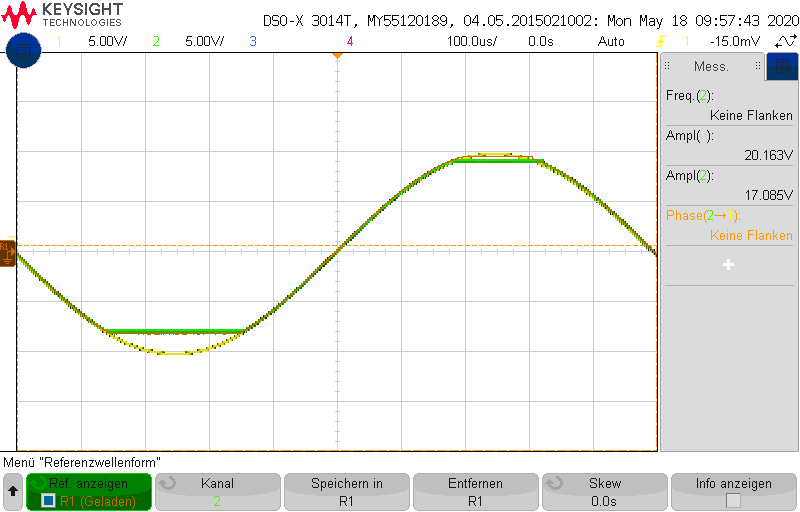
\includegraphics[width=0.8\textwidth]{Lab_1/Messungen/Folger/uberst-schw3.png}
    \caption{Aussteuerbereich $uA741$, $CH_{Ref}: R_{Last} = inf$, $CH_{2}: R_{Last} = 2k\Omega$}
    \label{fig:res_Folger_Aussteuerbereich}
\end{figure}
\begin{figure}[H]
    \centering
    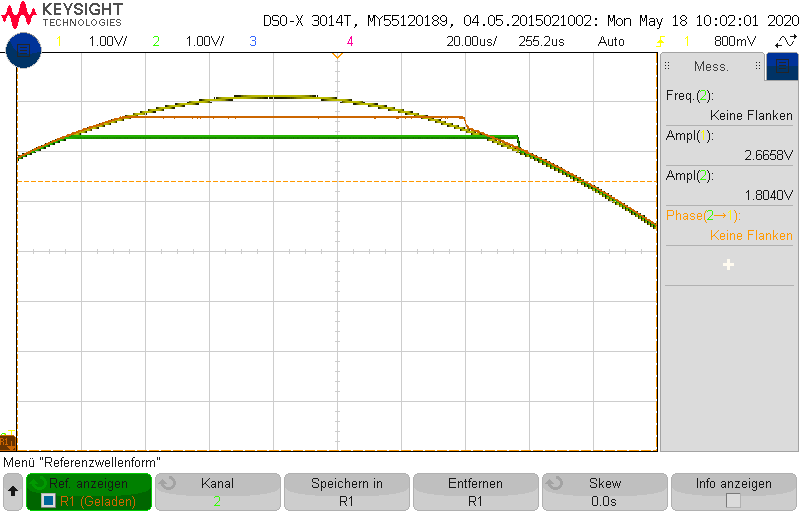
\includegraphics[width=0.8\textwidth]{Lab_1/Messungen/Folger/uberst-schw5.png}
    \caption{Aussteuerbereich Detailansicht $uA741$, $CH_{Ref}: R_{Last} = inf$, $CH_{2}: R_{Last} = 2k\Omega$}
    \label{fig:res_Folger_Aussterbereich_Detailansicht}
\end{figure}

\begin{figure}[H]
    \centering
    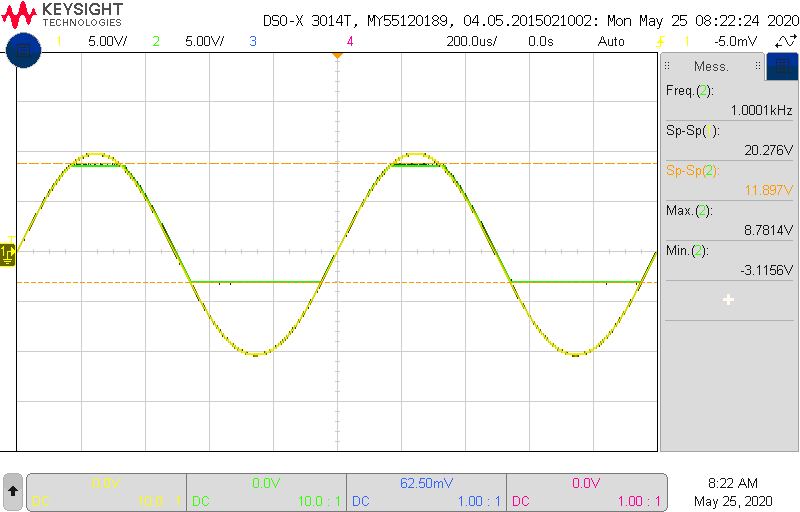
\includegraphics[width=0.8\textwidth]{Lab_1/Messungen/Folger/scope_5.png}
    \caption{Aussteuerbereich $uA741$, $CH_{Ref}: R_{Last} = inf$, $CH_{2}: R_{Last} = 2k\Omega$, $V_{CC} = 10V$, $V_{EE} = -5V$}
    \label{fig:res_Folger_VEE_M5V}
\end{figure}

\begin{figure}[H]
    \centering
    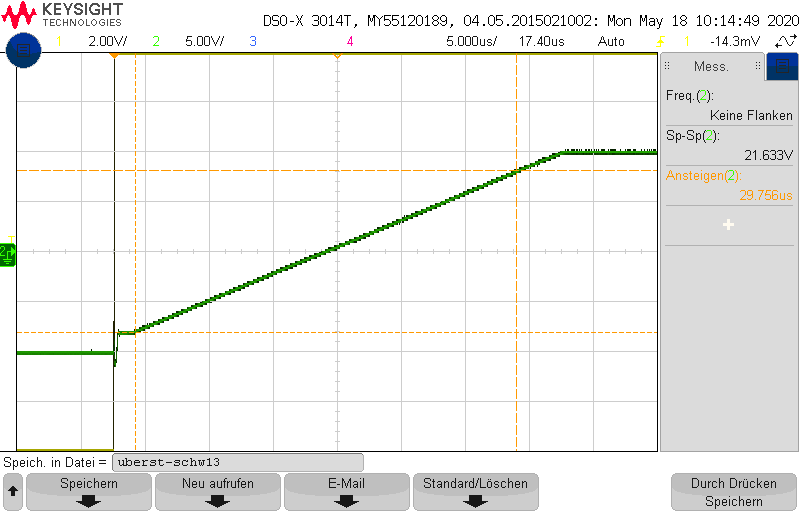
\includegraphics[width=0.8\textwidth]{Lab_1/Messungen/Folger/uberst-schw13.png}
    \caption{Slew Rate $uA741$, ohne kapazitive Last}
    \label{fig:res_Folger_Slew_rate}
\end{figure}

Mit den Messwerten aus \autoref{fig:res_Folger_Slew_rate} lässt sich nun eine Aussage über die Slew-Rate des Operationsverstärkers treffen. Hier muss beachtet werden, dass die Messfunktion \glqq Ansteigen\grqq des Oszilloskops bei dieser Messung von 10\% bis 90\% des maximalen Pegels des Signals gemessen hat. Das wurde in der Berechnung mit dem Korrekturfaktor 0,8 berücksichtigt. 

\begin{align}
    \.{u} &= \frac{U_{pp}}{t_{rise}} = \frac{21,633\V\cdot0,8}{29,759\us}\approx 0,582 \frac{\V}{\us}
\end{align}
Im Vergleich zum Datenblatt welches bei Unity-Gain eine typische Slewrate von $0,5\frac{\V}{\us}$ \cite[7]{ti:ua741} angibt, weißt dieser Wert keine signifikante Abweichung auf.

Daraus ergibt sich, dass für die maximale Amplitude die ohne überschreiten der maximalen Slew-rate folgendes gilt:
\begin{align}
    \hat{U}=\frac{\text{SLR}}{2\pi f_g}=\frac{0,582 \frac{\V}{\us}}{2\pi \cdot 826,48\kHz} =112,07\mV 
\end{align}
\begin{figure}[H]
    \centering
    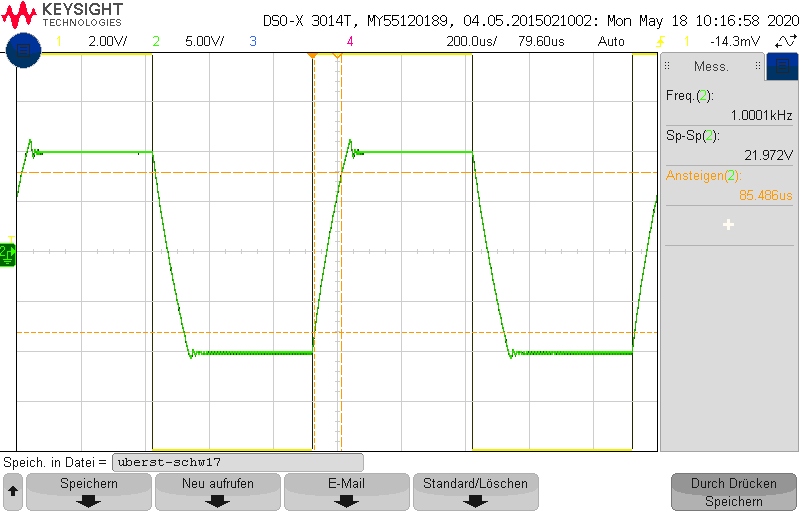
\includegraphics[width=0.8\textwidth]{Lab_1/Messungen/Folger/uberst-schw17.png}
    \caption{Slew Rate $uA741$,  mit kapazitiver Last}
    \label{fig:res_Folger_slew_rate_kap_last}
\end{figure}
Bei dieser Messung ist zu sehen, dass eine kapazitive Last zu einer stark vergrößerten Ansteigszeit und vermutlich wegen der parasitären Induktivität der Leitungen des Steckbretts zu einem Überschwingen nach Erreichen des oberen Aussteuerbereichs führt.

\subsection{Ausarbeitungen}
Der Ausgangs-Aussteuerbereich ist dadurch begrenzt, dass die Transistoren am Ausgang des OPVs nicht unbegrenzt niederohmig werden können. Desweiteren befinden sie sich irgendwann in Sättigung. An diesem Punkt kann die Spannung entlang der Kollektor-Emitter-Strecke nicht mehr kleiner werden. Außerdem befinden sich auf diesem Pfad ohmsche Verluste die auch mit steigender Stromstärke am Ausgang steigen.

Wie der Ausgangs-Aussteuerbereich ist auch der Gleichtaktaussteuerbereich der Schaltung durch die Versorgungsspannung und einer minimalen Differenz dazu vorgegeben.
%%%%%%%%%%%%%%%%%%%%%%%%%%%%%%%%%%%%%%%%%%%%%%%%%%%%%%%%%%%%%%%%%%%%%%%%%%%%%%%%%%%%%%%%%%%%%%%%%%%%%%%%%%%%%%%%%%%%%%%%%%%%%%%%%%%%
\section{Nicht invertierender Verstärker}
\subsection{Aufgabenstellung}
Es ist die Schaltung aus Abbildung \ref{fig:niinv_Verst_Schaltung} aufzubauen und mit  einer Verstärkung von $\nu=+10$ und $\nu = +101$ auszulegen. Dabei ist die Frequenz zu finden bei welcher der Verstärker das Signal aufgrund der Slew Rate verzerrt. 

Es sind die Frequenzgänge mit den beiden Verstärkungen aufzunehmen und mit der Verstärkung des geschlossenen Kreises zu vergleichen.

Die Kurve $U_a = f(U_e)$ der Schaltung mit $\nu=10$ ist mittels des X-Y-Betriebs des Oszilloskops aufzuzeichnen.

Das Verhalten bei rechteckförmigen Eingangsspannungen ist aufzunehmen.
\begin{figure}[H]
    \centering
    \begin{circuitikz}[]
        \draw (0,0) node[op amp,yscale=-1] (opamp) {\scalebox{1}[-1]{$\mu A 741$}};
        \draw (opamp.down) --++(0,0.5) node[vcc]{$V_{CC}$};
        \draw (opamp.up) --++(0,-0.5) node[vee]{$V_{EE}$};
        
        \draw (opamp.+) to[short,-o] ++(-2,0) node[left] {$U_{in}$};
        \draw (opamp.-) to[short] ++(-0.5,0)
            to[short] ++(0,-2.5)
            to[R=$R_1$] ++(0,-1.5) node[ground]{};
        \draw (opamp.out) to[short,-o] ++(2,0) node[right] {$U_a$};
        \draw (2,0) to[short,*-] ++(0,-2.5)
            to[R=$R_2$,-*] (-1.7,-2.5);
        \end{circuitikz}
    \caption{Nicht invertierender Verstärker}
    \label{fig:niinv_Verst_Schaltung}
 \end{figure}


\subsection{Auslegung der Schaltung}
\subsubsection{Verstärkung 10}
Zur Auslegung dieser Schaltung wurde zuerst ein Widerstand ausgewählt, damit wurde dann der Zweite berechnet.

\begin{align}
    \nu &= 1+ \frac{R_2}{R_1}\\
    R_2 &= 2k\Omega\\
    R_1 = R_2(\nu - 1) &= 18 k\Omega
\end{align}

\subsubsection{Verstärkung 101}

\begin{align}
    \nu &= 1+ \frac{R_2}{R_1}\\
    R_2 &= 1k\Omega\\
    R_1 = R_2(\nu - 1) &= 100 k\Omega
\end{align}

\subsection{Messaufbau}
Zur Aufnahme aller Messungen wurde sowohl die Ein- als auch die Ausgangsspannung mit dem Oszilloskop aufgenommen. Die Eingangsspannung wurde mit einem Signalgenerator erzeugt, dieser war im High-Z Modus. 
\begin{figure}[H]
    \centering
    \begin{circuitikz}[]
        \draw (0,0) node[op amp,yscale=-1] (opamp) {\scalebox{1}[-1]{$\mu A 741$}};
        \draw (opamp.down) --++(0,0.5) node[vcc]{$V_{CC}$};
        \draw (opamp.up) --++(0,-0.5) node[vee]{$V_{EE}$};
        
        \draw (opamp.-) to[short] ++(-0.5,0)
            to[short] ++(0,-2.5)
            to[R=$R_1$] ++(0,-1.5) node[ground]{};
        
        \draw (opamp.out) to[short,-o] ++(3,0)
            %Einfügen der Messchaltung
            to[sV=CH2, color=white, name=S2,o-o] ++(0,-2) node[ground]{};
        \draw (opamp.+) to[short,-o] ++(-2,0) 
            %%Einfügen der Messschaltung
            to[sV=CH1, color=white, name=S1,o-o] ++(0,-2) node[ground] {}
            to[short,o-] ++(-2,0)
            to[sV] ++(0,2)
            to[short,-o] ++(2,0);        
        \draw (2,0) to[short,*-] ++(0,-2.5)
            to[R=$R_2$,-*] (-1.7,-2.5);
            
        \myscope{S1}{0}
        \myscope{S2}{0}

        \end{circuitikz}
    \caption{Nicht invertierender Verstärker, Messaufbau}
    \label{fig:niinv_Verst_Schaltung_Messaufbau}
 \end{figure}


\subsection{Messergebnisse}
Wie in Abbildung \ref{fig:bode_niinv} zu erkennen ist, die Grenzfrequenz der Schaltung mit der höheren Verstärkung niedriger ist. Anhand des Gain-Bandwidth Produktes ist dieses Ergebnis nachvollziehbar. Es wurden keine signifikanten Abweichungen der Messungen von den Simulationen gefunden. 
\begin{figure}[H]
    \centering
    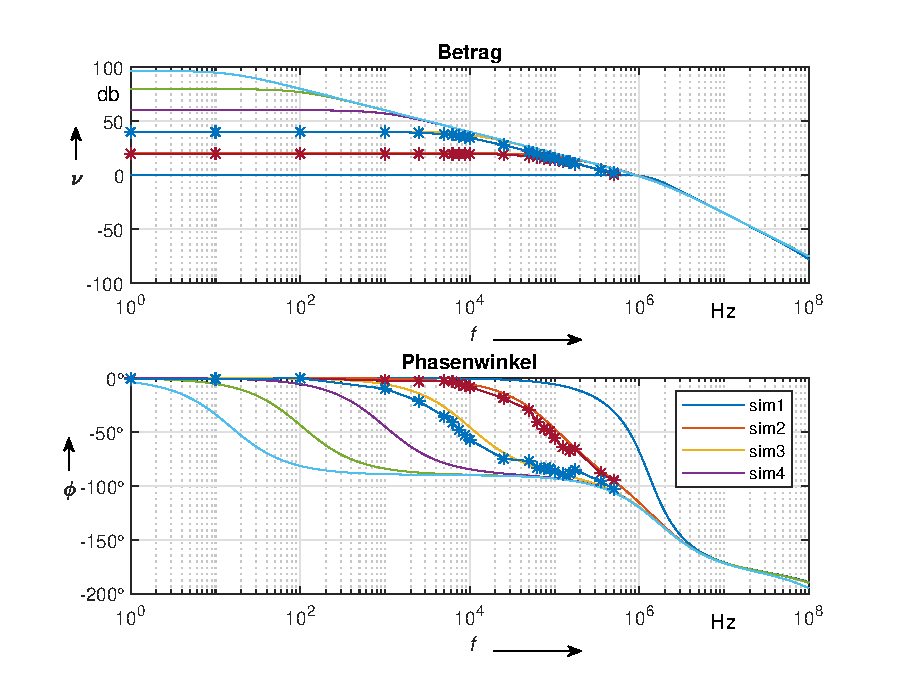
\includegraphics[width=\costumPlotWidth]{Lab_1/Plots/niinv_verst.eps}
    \caption{Bodediagramm nicht invertierender Verstärker}
    \label{fig:bode_niinv}
\end{figure}

\begin{figure}[H]
    \centering
    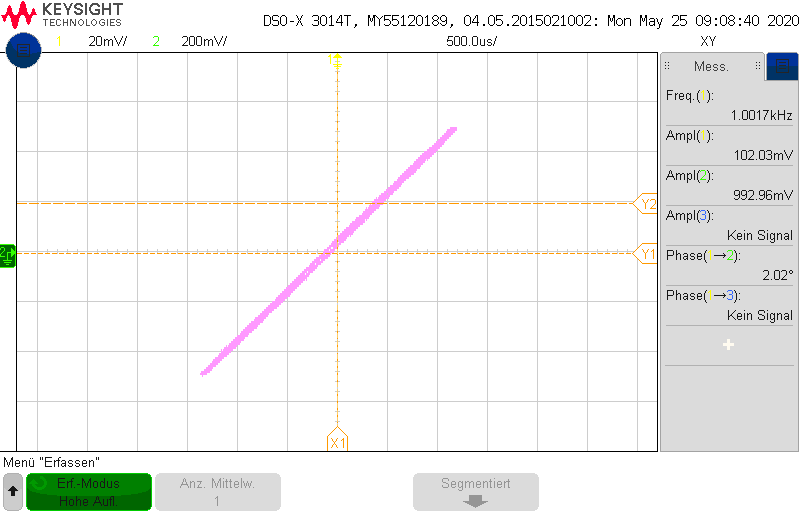
\includegraphics[width=\costumPicWidth]{Lab_1/Messungen/niinv_verst/xy_ohne_uebersteuern_1.png}
    \caption{$U_a = f(U_e)$ im XY Betrieb des Oszilloskops, ohne Übersteuern des Verstärkers }
    \label{fig:niinv_ohne_Uebersteuern}
\end{figure}
Bei positiver Eingangsspannung erzeugt ein nichtinvertierender Verstärker auch eine positive Ausgangsspannung, die höher ist als die Ausgangsspannung. Weil die Spannung an U+ und U- gleich sein ist, solange der Verstärker nicht übersteuert ist, fließt (bei einem unbelasteten Verstärker) der gesamte Ausgansstrom aus dem OPV durch die Rückkopplung $R_2$ und dann über $R_1$ auf Ground. Für negative Eingangsspannung ist es umgekehrt – der Strom fließt von Masse, durch die Rückkopplung, in den OPV.
\begin{figure}[H]
    \centering
    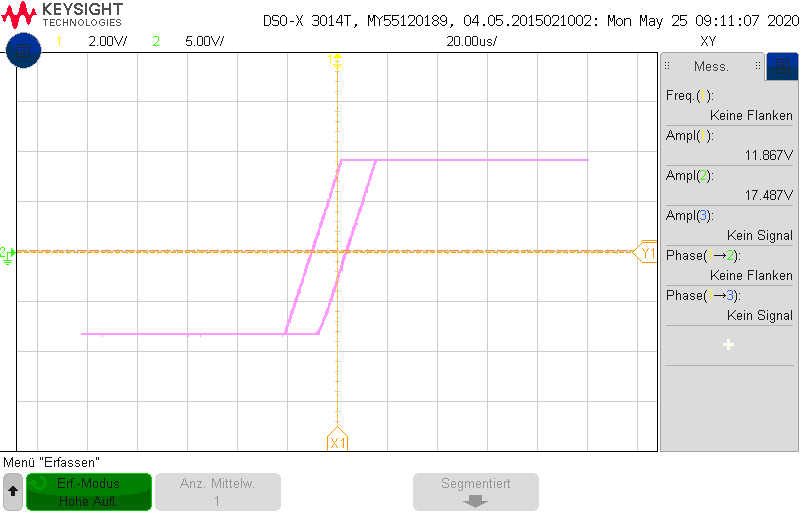
\includegraphics[width=\costumPicWidth]{Lab_1/Messungen/niinv_verst/xy_mit_uebersteuern_1.png}
    \caption{$U_a = f(U_e)$ im XY Betrieb des Oszilloskops, mit Übersteuern des Verstärkers}
    \label{fig:niinv_mit_Uebersteuern}
\end{figure}
An der positiven Steigung der Geraden in Abbildung \ref{fig:niinv_mit_Uebersteuern} und \ref{fig:niinv_ohne_Uebersteuern} sieht man dass die Schaltung das Eingangssignal nicht invertiert.

Bei negativer Eingangsspannung fließt eine Spannung in den Eingangspin des Verstärkers, bei positiver Spannung aus dem Pin heraus. 
\begin{figure}[H]
    \centering
    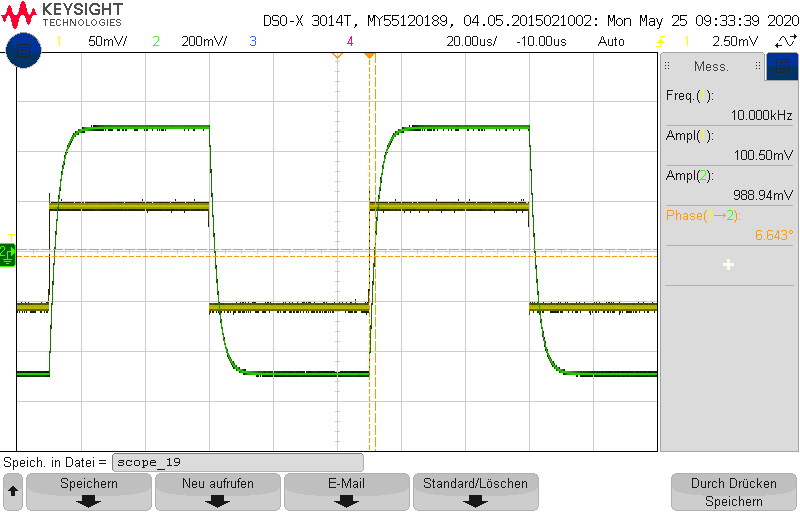
\includegraphics[width=\costumPicWidth]{Lab_1/Messungen/niinv_verst/square.png}
    \caption{Rechteckige Eingangsspannung}
    \label{fig:niinv_rechteck}
\end{figure}
Auch hier ist zu erkennen, dass bei größerer Verstärkung bereits bei deutlich niedrigern Frequenzen ein Tiefpassverhalten auftritt.

\subsection{Ausarbeitungen}
Der Eingangswiderstand dieser Schaltung wäre bei einem idealen OPamp unendlich groß. Bei dieser Schaltung wird (bei weitem :D) kein idealer Operationsverstärker verwendet, das heißt der Eingangswiderstand der Schaltung entspricht dem Eingangswiderstand des nicht-invertierenden Pins des Verstärkers. Dieser ist zwar groß und befindet sich im Bereich $R_{in}=1\MOhms-300\KOhms$, aber nicht unendlich groß. Um einen definierten Eingagswiderstand zu erhalten, müsste ein paralleler Widerstand (z.B. $R_{in}=50\Omega$) eingesetzt werden. Der dazu parallele Eingangswiderstand des Operationsverstärkers kann wegen seine Größe in den allermeisten Fällen vernachlässigt werden.


In \autoref{fig:niinv_mit_Uebersteuern} ist erkennbar, dass die maximale Aussteuerung bei 13,153V liegt, begrenzt durch den negativen Bereich. Für die Berechnung der Großsignalbandbreite wird abhängig von diesem Wert davon ausgegangen, dass die maximale Aussteuerung ohne Verzerrung bei einer Amplitude 13V liegt.
Gemessen wurde bis zu einer Frequenz von $f_{Meas}=300\kHz$. Dabei war die gemessene Verstärkung für $\nu_{\text{Durchlassvbereich}}=8,5dB$  und für $\nu_{\text{Durchlassvbereich}}=101$ noch $7,7dB$.

\begin{align}
    8,5\dB \longrightarrow 10^\frac{8,5}{20}=  2,6607\longrightarrow \text{GBW}=300\kHz\cdot 2,6607=798,21\kHz \\
    7,7\dB \longrightarrow 10^\frac{7,7}{20}=  2,4266\longrightarrow \text{GBW}=300\kHz\cdot 2,6607=727,98\kHz 
\end{align}
Laut Datenblatt ist der typische Wert für einen UA741 1MHz, minimal 700kHz. Diese Werte stimmen mit den gemessenen Ergebnissen überein. Für die Berechnung der Frequenz wird der niedrigere der beiden gemessenen Werte verwendet
\begin{align}
    f_{Max}=\frac{\text{GBW}}{2\pi \hat{U}_a} =\frac{727,98\kHz}{2\pi13\V}=8,912\kHz
\end{align}
Bei einer Amplitude von 13V kann bei einem angenommenen Gain-Bandwidth-Product von $727,98\kHz$ das Signal bis zu einer maximalen Frequenz von $8,912\kHz$ unverzerrt wiedergegeben werden.

\section{Invertierender Verstärker}
\subsection{Aufgabenstellung}
Die Schaltung aus Abbildung \ref{fig:inv_verst_Schaltung} ist für eine Verstärkung $\nu = -10$ und $\nu=-100$auszulegen und auf dem Steckbrett aufzubauen. Von diesen beiden Schaltungen ist das Bodediagramm aufzunehmen und mit einer Simulation zu vergleichen.

Es ist zu dokumentieren was am virtuellen Nullpunkt der Schaltung bei Übersteuerung des Ausgangs passiert. Diese Messung ist bei einer Frequenz von $f=1kHz$ durchzuführen. 

Mittels des XY-Betriebs ist zu zeigen, in welche Richtung der Strom am OPamp Ausgangspin fließt bei positiven und negativen Ausgangsspannungen. 

\begin{figure}[H]
    \centering
    \begin{circuitikz}[]
        %%Verstärker und Versorgung
        \draw (0,0) node[op amp] (opamp) {$\mu A 741$};
        \draw (opamp.up) --++(0,0.5) node[vcc]{$V_{CC}$};
        \draw (opamp.down) --++(0,-0.5) node[vee]{$V_{EE}$};
        
        \draw (opamp.+) to[short] ++(-0.25,0)
            to[short] ++(0,-0.25) node[ground] {};
        
        \draw (opamp.-) to[short] (-2,0.5)
            to[R=$R_1$,*-o] ++(-2,0) node[left] {$U_{in}$};
        \draw (-2,0.5) to[short] ++(0,2)
            to[R=$R_2$] ++(4,0)
            to[short,-*] ++(0,-2.5);
        \draw (opamp.out) to[short,-o] ++(2,0) node[right] {$U_a$};
        \end{circuitikz}
    \caption{Invertierender Verstärker}
    \label{fig:inv_verst_Schaltung}
 \end{figure}

\subsection{Messaufbau}
Zur Aufnahme aller Messungen wurde sowohl die Ein- als auch die Ausgangsspannung mit dem Oszilloskop aufgenommen. Die Eingangsspannung wurde mit einem Signalgenerator erzeugt, dieser war im High-Z Modus. 
\begin{figure}[H]
    \centering
    \begin{circuitikz}[]
        %%Verstärker und Versorgung
        \draw (0,0) node[op amp] (opamp) {$\mu A 741$};
        \draw (opamp.up) --++(0,0.5) node[vcc]{$V_{CC}$};
        \draw (opamp.down) --++(0,-0.5) node[vee]{$V_{EE}$};
        
        \draw (opamp.+) to[short] ++(-0.25,0)
            to[short] ++(0,-0.25) node[ground] {};
        
        \draw (opamp.-) to[short] (-2,0.5)
            to[R=$R_1$,*-o] ++(-2,0)
            %%Einfügen der Messschaltung
            to[sV=CH1, color=white, name=S1,o-o] ++(0,-2) node[ground] {}
            to[short,o-] ++(-2,0)
            to[sV] ++(0,2)
            to[short,-o] ++(2,0);        
        \draw (-2,0.5) to[short] ++(0,2)
            to[R=$R_2$] ++(4,0)
            to[short,-*] ++(0,-2.5);
        \draw (opamp.out) to[short,-o] ++(2,0)        
            %Einfügen der Messchaltung
            to[sV=CH2, color=white, name=S2,o-o] ++(0,-2) node[ground]{};
        \myscope{S1}{0}
        \myscope{S2}{0}
        \end{circuitikz}
    \caption{Invertierender Verstärker, Messaufbau}
    \label{fig:inv_verst_Schaltung_Messaufbau}
 \end{figure}


\subsection{Auslegung}
\begin{align}
    \nu = -\frac{R_2}{R_1} =-10 \longrightarrow R_2 = 10R_1=10\cdot 10\KOhms =100\KOhms
\end{align}
\subsection{Messergebnisse}
\begin{figure}[H]
    \centering
    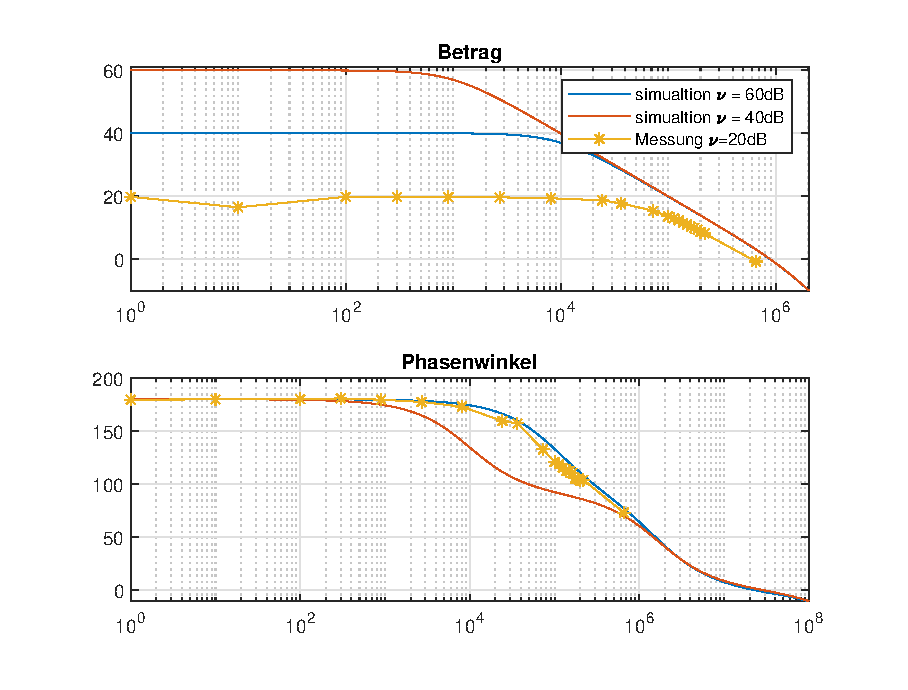
\includegraphics[width=\costumPicWidth]{Lab_1/Plots/inv_verst.eps}
    \caption{Bodediagramm invertierender Verstärker}
    \label{fig:bode_inv_verst}
\end{figure}
Solange die Verstärkerschaltung nicht übersteuert, regelt der OPV die Eingangsspannungen (ideal betrachtet) auf
den gleichen Wert, also U+ = U-. Wenn übersteuert wird, funktioniert diese Regelung nicht mehr. Statt dem
virtuellen Nullpunkt ist am invertierenden Eingang dann die Differenz-Spannung zwischen tatsächlichem und
möglichem Eingangs-Wert vorhanden.
\begin{figure}[H]
    \centering
    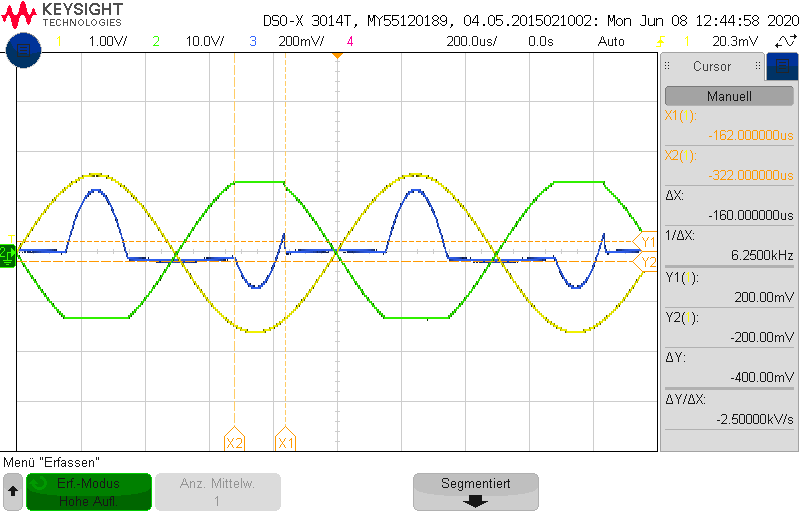
\includegraphics[width=\costumPicWidth]{Lab_1/Messungen/inv_verst/scope_40.png}
    \caption{Invertierender Verstärker bei Übersteuerung}
    \label{fig:uberst_verst}
\end{figure}
Eine negative Ausgangsspannung bedeutet, dass am Ausgang des OPVs eine positive Spannung entsteht. Diese
Spannung lässt über R2 zum virtuellen Nullpunkt einen Strom fließen, der aus dem OPV kommt. Für positive
Eingangsspannung ist der Ausgang negativ, also fließt ein Strom durch die Rückkopplung in den OPV hinein.
\begin{figure}[H]
    \centering
    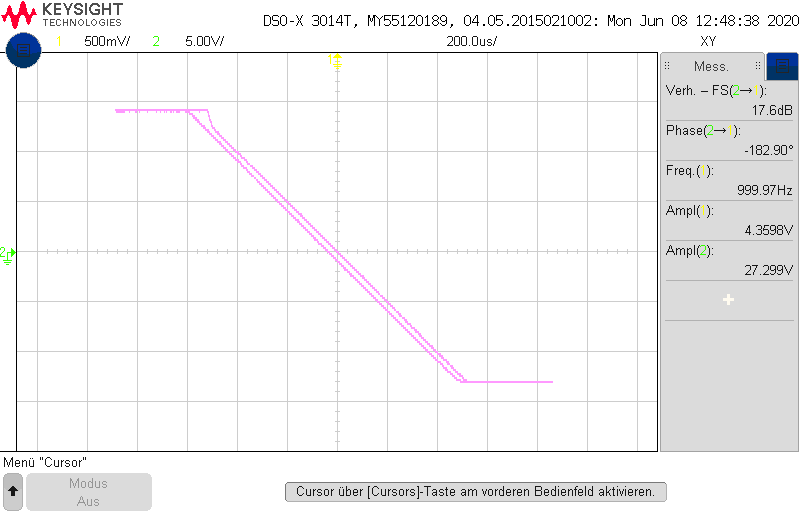
\includegraphics[width=\costumPicWidth]{Lab_1/Messungen/inv_verst/scope_48.png}
    \caption{Invertierender Verstärker dargestellt im X-Y Betrieb des Osilloskop}
    \label{fig:inv_verst_xy}
\end{figure}

\subsection{Ausarbeitungen}
Der Eingangswiderstand dieser Schaltung ist $R_1$. Da beim OPamp im Idealfall an beiden Eingangspins die gleiche Spannung anliegen soll, liegt am virtuellen Nullpunkt das GND Potential an. Daraus ergibt sich, dass $R_1$ der Eingangswiderstand der Schaltung ist.

Der nichtinvertierende Eingang liegt auf Ground, also liegt auch der Mittelwert von U+ und U- bei 0V. Damit beträgt die Gleichtaktaussteuerung bei dieser Schaltung 0V.
\section{Addierschaltung}
\subsection{Aufgabenstellung}
Die Schaltung aus dem vorherigen Kapitel ist mit einem weitern Eingang zu erweitern. Danach sind zwei verschiedene Wechselspannungen anzulegen. Eine davon sollte einen Gleichspannungsoffset aufweisen. 
\begin{figure}[H]
    \centering
    \begin{circuitikz}[]
        %%Verstärker und Versorgung
        \draw (0,0) node[op amp] (opamp) {$\mu A 741$};
        \draw (opamp.up) --++(0,0.5) node[vcc]{$V_{CC}$};
        \draw (opamp.down) --++(0,-0.5) node[vee]{$V_{EE}$};
        
        \draw (opamp.+) to[short] ++(-0.25,0)
            to[short] ++(0,-0.25) node[ground] {};
        
        \draw (opamp.-) to[short] (-2,0.5)
            to[R=$R_1$,*-o] ++(-2,0) node[left] {$U_{in1}$};
        \draw (-2,2.5) to[R=$R_2$,*-o] ++(-2,0) node[left] {$U_{in2}$};
        \draw (-2,0.5) to[short] ++(0,2)
            to[R=$R_{ref}$] ++(4,0)
            to[short,-*] ++(0,-2.5);
        \draw (opamp.out) to[short,-o] ++(2,0) node[right] {$U_a$};
        \end{circuitikz}
    \caption{Addierschaltung}
    \label{fig:Addierschaltung}
 \end{figure}


\subsection{Messaufbau}
Zur Aufname aller Messungen wurde ein anderer Signalgenerator als im Labor vorhanden war. Ich habe in dieser Laborübung meinen eigenen mitgebracht. Dieser hat den Vorteil, dass er zwei synchronisierte Ausgänge besitzt. Alle Ein- und Ausgänge wurden mit dem Oszilloskop aufgenommen
\begin{figure}[H]
    \centering
    \begin{circuitikz}[]
        %%Verstärker und Versorgung
        \draw (0,0) node[op amp] (opamp) {$\mu A 741$};
        \draw (opamp.up) --++(0,0.5) node[vcc]{$V_{CC}$};
        \draw (opamp.down) --++(0,-0.5) node[vee]{$V_{EE}$};
        
        \draw (opamp.+) to[short] ++(-0.25,0)
            to[short] ++(0,-0.25) node[ground] {};
        
        \draw (opamp.-) to[short] (-2,0.5)
            to[R=$R_1$,*-o] ++(-2,0) to[short] ++(-1,0)             
            %%Einfügen der Messschaltung
            to[sV=CH3, color=white, name=S3,*-*] ++(0,-2) node[ground] {}
            to[short,*-] ++(-2,0)
            to[sV] ++(0,2)
            to[short,-*] ++(2,0);     
        \draw (-2,2.5) to[R=$R_2$,*-o] ++(-2,0) to[short] ++(-4,0)            
        %%Einfügen der Messschaltung
            to[sV=CH1, color=white, name=S1,*-*] ++(0,-2) node[ground] {}
            to[short,*-] ++(-2,0)
            to[sV] ++(0,2)
            to[short,-*] ++(2,0);     ;
        \draw (-2,0.5) to[short] ++(0,2)
            to[R=$R_{ref}$] ++(4,0)
            to[short,-*] ++(0,-2.5);
        \draw (opamp.out) to[short,-o] ++(2,0)            
        to[sV=CH2, color=white, name=S2,o-o] ++(0,-2) node[ground]{};

        \myscope{S1}{0}
        \myscope{S2}{0}
        \myscope{S3}{0}
        \end{circuitikz}
    \caption{Addierschaltung Messaufbau}
    \label{fig:Addierschaltung_Messaufbau}
 \end{figure}


\subsection{Messergebnisse}
Zur besseren Darstellung der Addition wurden hier Sinusspannungen mit zwei verschiedenen Frequenzen angelegt. Das Ergebnis entsprach den Erwartungen. 
\begin{figure}[H]
    \centering
    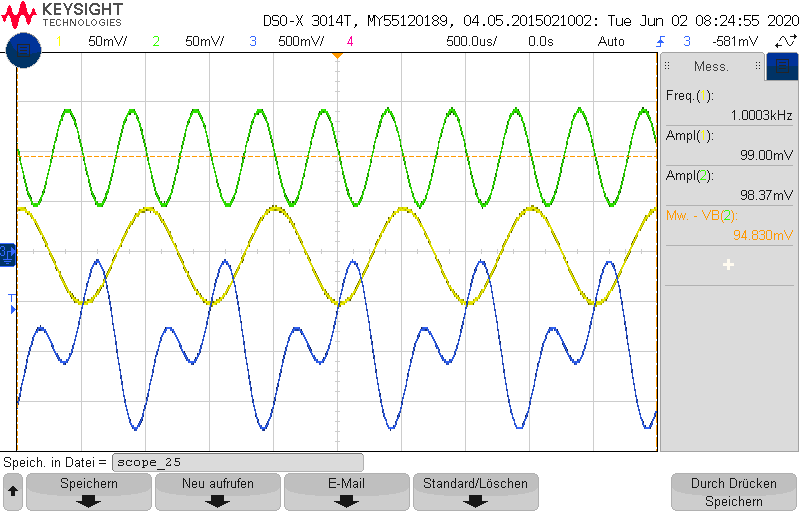
\includegraphics[width=\costumPicWidth]{Lab_1/Messungen/Addierer/scope_25.png}
    \caption{Addition zweier Sinusspannungen}
    \label{fig:Addierschaltung_Ergebnis}
\end{figure}

\section{Geräteverzeichnis}
\begin{table}[H]
\centering
\caption{Geräteverzeichnis 1. Übung}
\label{tab:Gerteverzeichnis}
\begin{tabular}{|
>{\columncolor[HTML]{C0C0C0}}l |l|l|l|}
\hline
Gerät           & \cellcolor[HTML]{C0C0C0}Hersteller & \cellcolor[HTML]{C0C0C0}Bezeichnung & \cellcolor[HTML]{C0C0C0}Seriennummer \\ \hline
Multimeter      & Agilent                            & 34450A                              & 9949728                              \\ \hline
Netzteil        & TTI                                & PL303QMD                            & 9949264                              \\ \hline
Signalgenerator & Keysight                           & 33500B Series                       & 9949719                              \\ \hline
Oszilloskop     & Keysight                           & DSO-X 3014T                         & 9949710                              \\ \hline
\end{tabular}
\end{table}